\documentclass[preprint,12pt]{elsarticle}

%% Use the option review to obtain double line spacing
%% \documentclass[authoryear,preprint,review,12pt]{elsarticle}

%% Use the options 1p,twocolumn; 3p; 3p,twocolumn; 5p; or 5p,twocolumn
%% for a journal layout:
%% \documentclass[final,1p,times]{elsarticle}
%% \documentclass[final,1p,times,twocolumn]{elsarticle}
%% \documentclass[final,3p,times]{elsarticle}
%% \documentclass[final,3p,times,twocolumn]{elsarticle}
%% \documentclass[final,5p,times]{elsarticle}
%% \documentclass[final,5p,times,twocolumn]{elsarticle}

%% For including figures, graphicx.sty has been loaded in
%% elsarticle.cls. If you prefer to use the old commands
%% please give \usepackage{epsfig}

%% The amssymb package provides various useful mathematical symbols
\usepackage{amssymb}
%% The amsthm package provides extended theorem environments
%% \usepackage{amsthm}

%% The lineno packages adds line numbers. Start line numbering with
%% \begin{linenumbers}, end it with \end{linenumbers}. Or switch it on
%% for the whole article with \linenumbers.
%% \usepackage{lineno}

\usepackage{units}
\usepackage{gensymb}
\usepackage{graphicx}
\usepackage{booktabs}
\graphicspath{{Figures/}}


\usepackage{booktabs} %%% scientific publication style tables
%\usepackage{empheq}   %%% for boxed equations and alike
%\usepackage{xcolor}   %%% for colored text and formulae
\usepackage{amsmath}  %%% math symbols needed
\usepackage{amsfonts} %%% math fonts needed
\usepackage{amssymb}  %%% maths symbols needed 
\usepackage{amsthm}   %%% theorem environments
%\usepackage{dsfont}   %%% for blackboard numbers and characters 
\usepackage{float}   
\usepackage[]{hyperref} 
%\usepackage{subfigure} 
\usepackage{subcaption}
\usepackage{caption}   
\usepackage[utf8]{inputenc}
\usepackage[T1]{fontenc}
%\usepackage{helvet}

\usepackage{siunitx}
\usepackage[above]{placeins}
\usepackage{stfloats}

\usepackage[italic]{hepnames}
\usepackage[final]{pdfpages} %set to "final" in the end to show the pdf page
%\usepackage{pifont}
\usepackage{setspace}
\usepackage{textcomp}

\usepackage{natbib} % Order the citations

\bibliographystyle{unsrtnat}


%\newcommand{\degree}{\ensuremath{^\circ}}
\newcommand{\redcomment}[1]{\ding{110}\ding{43}\textcolor{red}{#1}}

\newcommand{\geant}{\textsc{Geant4}\xspace}
\newcommand{\slic}{\textsc{SLIC}\xspace}
\newcommand{\lcsim}{\texttt{org.lcsim}\xspace}
\newcommand{\gdml}{\textsc{GDML}\xspace}
\newcommand{\vrml}{\textsc{VRML}\xspace}
\newcommand{\xml}{\textsc{XML}\xspace}
\newcommand{\lcdd}{\textsc{LCDD}\xspace}
\newcommand{\lcio}{\textsc{LCIO}\xspace}
\newcommand{\ilcsoft}{\textsc{ILCSoft}\xspace}
\newcommand{\marlin}{\textsc{Marlin}\xspace}
\newcommand{\Root}{\textsc{ROOT}\xspace}
\newcommand{\Cplusplus}{\texttt{C++}\xspace}


\journal{Nuclear Physics B}




\begin{document}

\begin{frontmatter}

%% Title, authors and addresses

%% use the tnoteref command within \title for footnotes;
%% use the tnotetext command for theassociated footnote;
%% use the fnref command within \author or \address for footnotes;
%% use the fntext command for theassociated footnote;
%% use the corref command within \author for corresponding author footnotes;
%% use the cortext command for theassociated footnote;
%% use the ead command for the email address,
%% and the form \ead[url] for the home page:
%% \title{Title\tnoteref{label1}}
%% \tnotetext[label1]{}
%% \author{Name\corref{cor1}\fnref{label2}}
%% \ead{email address}
%% \ead[url]{home page}
%% \fntext[label2]{}
%% \cortext[cor1]{}
%% \address{Address\fnref{label3}}
%% \fntext[label3]{}

\title{Simulation of DESY-II Test Beam Facility}

%% use optional labels to link authors explicitly to addresses:
%% \author[label1,label2]{}
%% \address[label1]{}
%% \address[label2]{}

\author[Glasgow]{F.~Jöhlinger}
\author[desy]{A.~Schütz}
\author[desy]{M.~Stanitzki}
\address[desy]{DESY, Notkestrasse 85, D-22607 Hamburg}
\address[Glasgow]{University of Glasgow}

\begin{abstract}
DESY (Deutsches Elektronen-Synchrotron) is operating the DESY-II Test Beam 
Facility, one of the few test beam lines available in the world. To provide the 
users with an accurate simulation package of the beam line properties and to 
support further developments for the beam line itself, 
a flexible simulation package based on \slic and \geant simulation packages was developed.  
The package simulates the entire beam line from the beam generation in the 
DESY-II synchrotron down to all individual elements in the beam line. The 
results from this complete simulation are presented, including particle rates, beam 
momentum spread and backgrounds.

\end{abstract}

\begin{keyword}
%% keywords here, in the form: keyword \sep keyword

%% PACS codes here, in the form: \PACS code \sep code

%% MSC codes here, in the form: \MSC code \sep code
%% or \MSC[2008] code \sep code (2000 is the default)

\end{keyword}

\end{frontmatter}

%% \linenumbers

%% main text









\chapter{Introduction}
\label{Introduction}
\todo{Write an introduction}

\section{The DESY-II test beam simulation}
\subsection{Software used for the simulation toolkit}
The simulation of the DESY-II test beam generation was done using 
\slic~\cite{Graf:2006ei,slic}, a full simulation package that uses the \geant \cite{Agostinelli2003250,1610988} detector 
simulation toolkit. As mentioned previously, the test beam generation involves  
several steps, each of which involves certain beam line components. The 
components' geometry is defined in a \gdml (Geometry Description Markup 
Language) file, which allows the description of detector geometries with 
arbitrary placements~\cite{gdml}. A so-called compact \xml file, to which the 
\gdml file is linked, contains additional information about the world volume, 
tracking volume and other self defined logical volumes. Magnetic fields and 
various kinds of sensitive detector parts, which can be set up to simulate 
particle detectors, are specified in the compact file as well. 
The \xml compact file and the \gdml file are then compiled into the  \lcdd~(``Linear Collider Detector Description)~\cite{McCormick:2005jc} file format, as \geant requires all 
information about the geometry, the fields and sensitive detector parts sorted 
by the solid, the physical volume and the logical volume. The conversion using 
the \textit{detector-framework} software package from the \lcsim (Linear Collider 
Simulation) framework expands the basic information of the detector components 
into the verbose and hierarchical style that is required for \geant. \\ \slic's 
stores the output of the simulation using th  \lcio (Linear Collider 
Input/Output) format~\cite{Aplin:2012kj,LCIO_DOC}.

\subsection{Event generation for DESY-II beam bunch}
The first step in the chain of the test beam generation is the DESY-II beam 
bunch consisting of 10$^{10}$ electrons or positrons hitting a primary target 
placed directly in the beam pipe. 
Thi uses the  average properties of a  DESY-II bunch, like the beam bunch size 
and its energy distribution.
\slic uses the \geant physics list \textit{LCPhys}~\cite{SLIC_LCPhys} 
, which contains several classes for gamma, lepton, hadron and 
ion physics as well as particle decays.

The energy and spatial distribution of the simulated DESY-II synchrotron beam is shown in Figure~\ref{fig:DESY-II_beam_bunch_energy_spacial_deflection}.

\begin{figure}
  \centering
  \begin{subfigure}[t]{0.47\textwidth}
    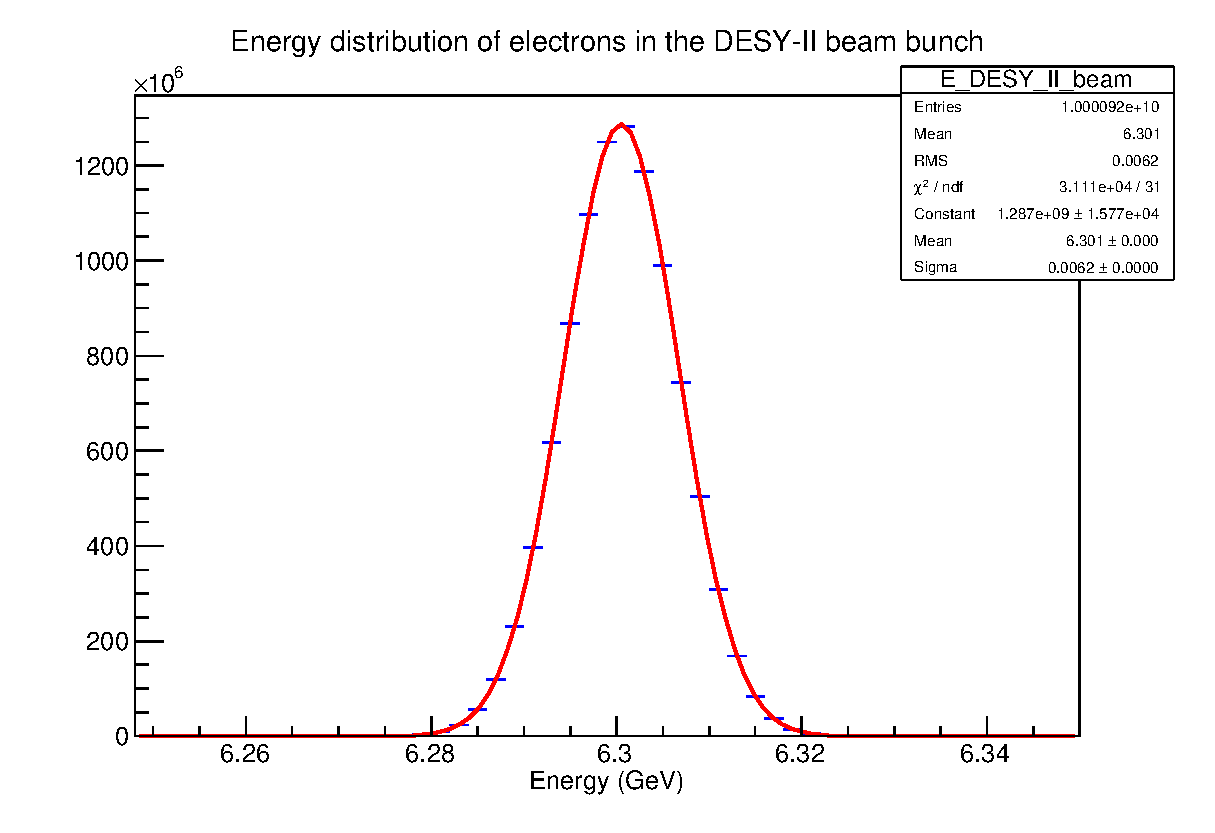
\includegraphics[width=\textwidth]{beam_Energy_Canvas_withFitParameters.eps}
      \caption[Energy distribution of DESY-II beam bunch.]{Energy distribution of the DESY-II beam bunch. A bunch contains 10$^{10}$ electrons with a mean energy of 6.301\,GeV. The Gaussian distribution has a sigma value of $\sigma_E$=0.0062\,GeV=6.2\,MeV.}
  \end{subfigure}
\hfill
  \begin{subfigure}[t]{0.47\textwidth}
    \includegraphics[width=\textwidth]{beam_Position_Canvas.jpg}
      \caption[Spacial distribution of electrons in DESY-II beam bunch.]{Spacial distribution of the electrons in the DESY-II beam bunch at ring position of test beam generation for test beam line 21. The horizontal and vertical beam sizes are calculated as $\sigma_y$=1.534\,mm and $\sigma_y$=0.753\,mm.}
  \end{subfigure}
 \caption[Simulated DESY-II beam bunch: energy and spacial distribution of electrons.]{The energy and spacial distribution of the simulated 10$^{10}$ electrons in the DESY-II beam bunch.}
  \label{fig:DESY-II_beam_bunch_energy_spacial_deflection}
\end{figure}

\subsection{The test beam primary target}

The primary target of the DESY-II test beam lines is a carbon fibre of 25(NOTE, 
actually more like 6-7) \,\textmu m thickness. When the simulated DESY-II beam 
bunch hits the fibre, bremsstrahlung photons are emitted, their energy 
distribution which follows the characteristic $\frac{1}{E}$ dependency 
of bremsstrahlung spectra is shown in Figure~\ref{fig:bremsstrahlung_spectrum}.

\begin{figure}[htbp]
  \centering
    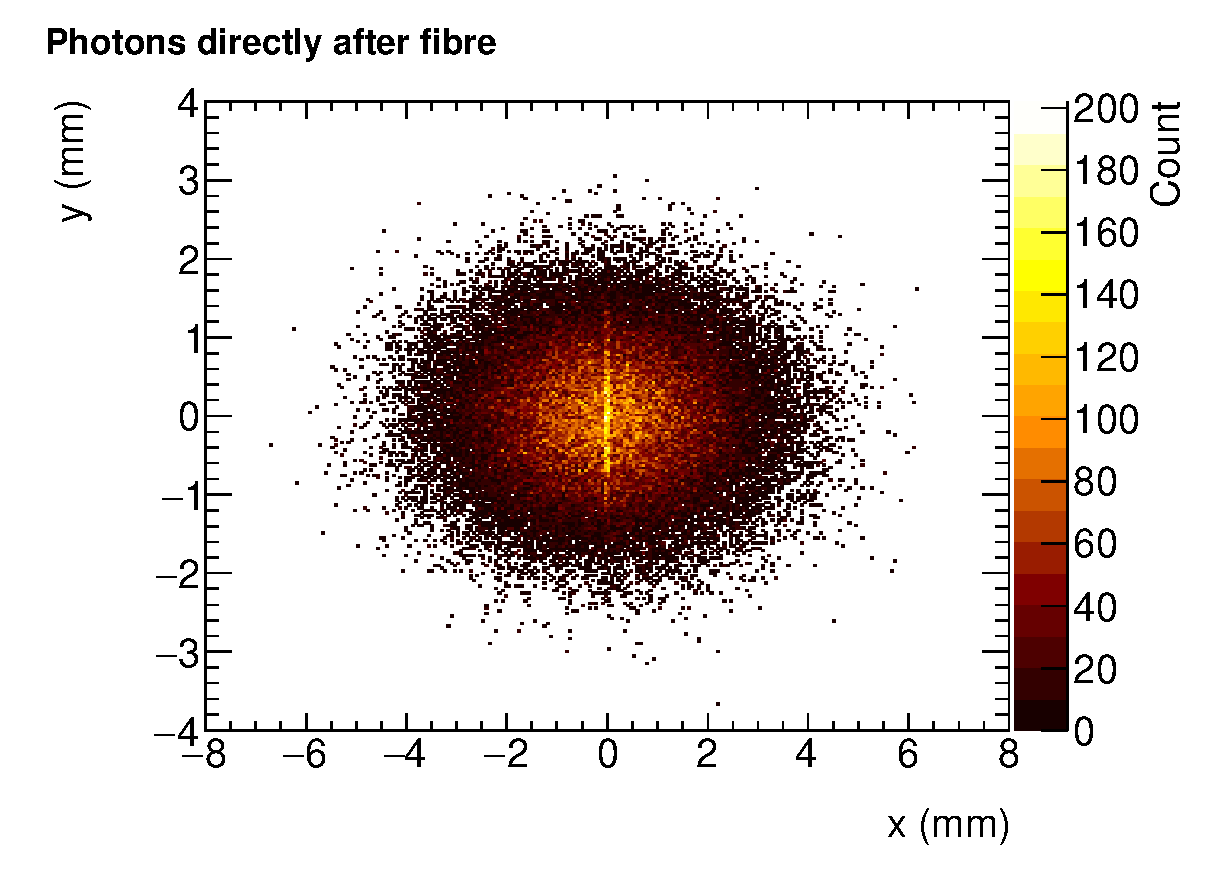
\includegraphics[width=0.8\textwidth]{Photons_after_Fibre_bigger_world_large.eps}
  \caption[Simulated bremsstrahlung photons emitted from the primary target.]{The DESY-II beam bunch hits the primary target and emits bremsstrahlung photons. The carbon fibre as well as the dimensions and shape of the beam bunch are clearly visible.}
  \label{fig:bremsstrahlung_scatter}
\end{figure}

\begin{figure}[htbp]
  \centering
    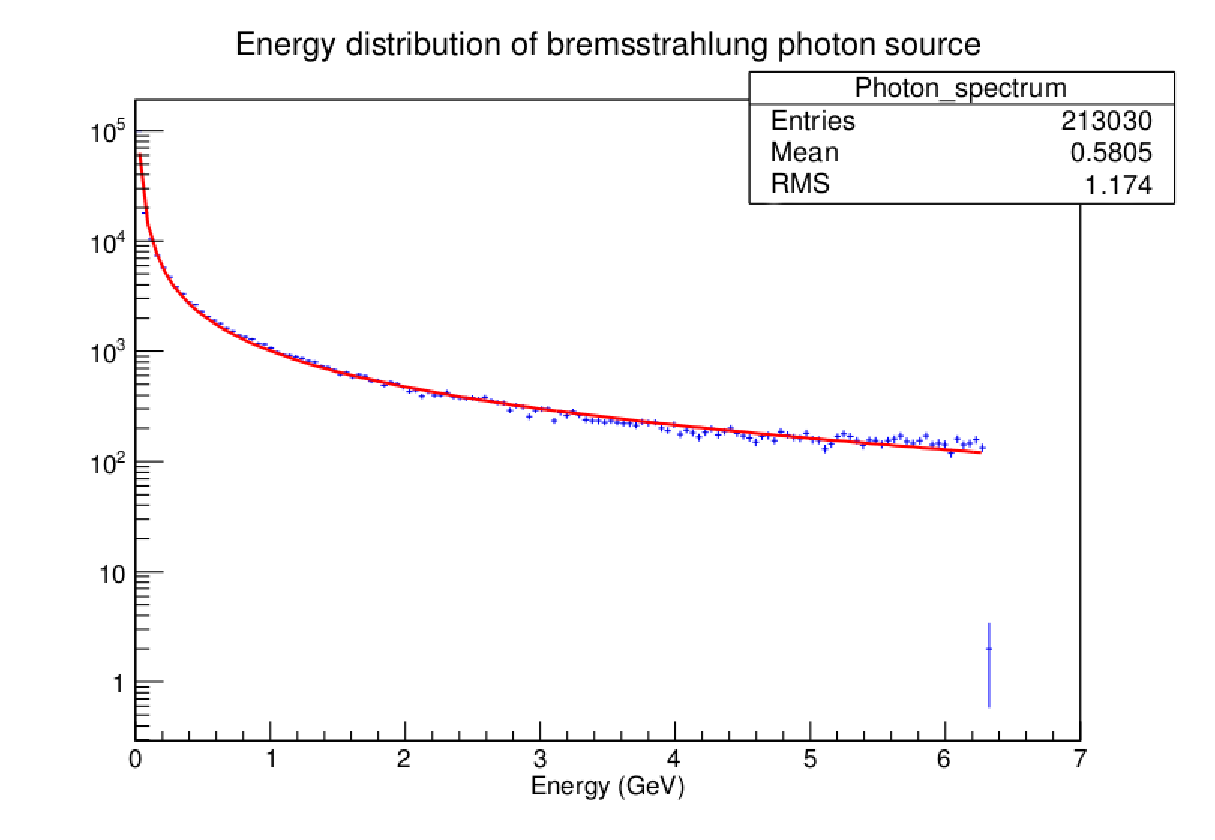
\includegraphics[width=\textwidth]{bremsstrahlungSpectrum_wo_Chi2.eps}
  \caption[Simulated bremsstrahlung spectrum emitted from the primary target.]{The DESY-II beam bunch of 10$^{10}$ electrons generates in total about $2\cdot10^5$ bremsstrahlung photons by hitting the primary target. The bremsstrahlung spectrum reaches to about 6.3\,GeV, which is the maximum energy of the photons, as they cannot exceed the maximum energy of the respective electrons. Mostly low energy photons in the MeV range are produced.}
  \label{fig:bremsstrahlung_spectrum}
\end{figure}

% The number of emitted photons in a certain energy range, between $k_{min}$ and $k_{max}$, can be expressed with the following equation for the case of a very thin target ($dt\rightarrow d\ll X_0$) \cite[page 405]{PDG}:
% \begin{equation}
%  N_{\gamma}=\frac{d}{X_0}\left[\frac43ln\left(\frac{k_{max}}{k_{min}}\right)-\frac{4(k_{max}-k_{min})}{3E}+\frac{k_{max}^2-k_{min}^2}{2E^2}\right]
%  \label{eq:bremsstrahlung_spectrum_2}
% \end{equation}

 
As the bremsstrahlung photons can only exit the beam pipe tangentially to DESY-II 
synchrotron ring, the further test beam line components are placed along the 
beam path of the bremsstrahlung photons. A map of the DESY-II test beam facility with its three test beam lines are 
shown in Figure~\ref{fig:Test Beam Lines}.

\begin{figure}[ht]
  \centering
  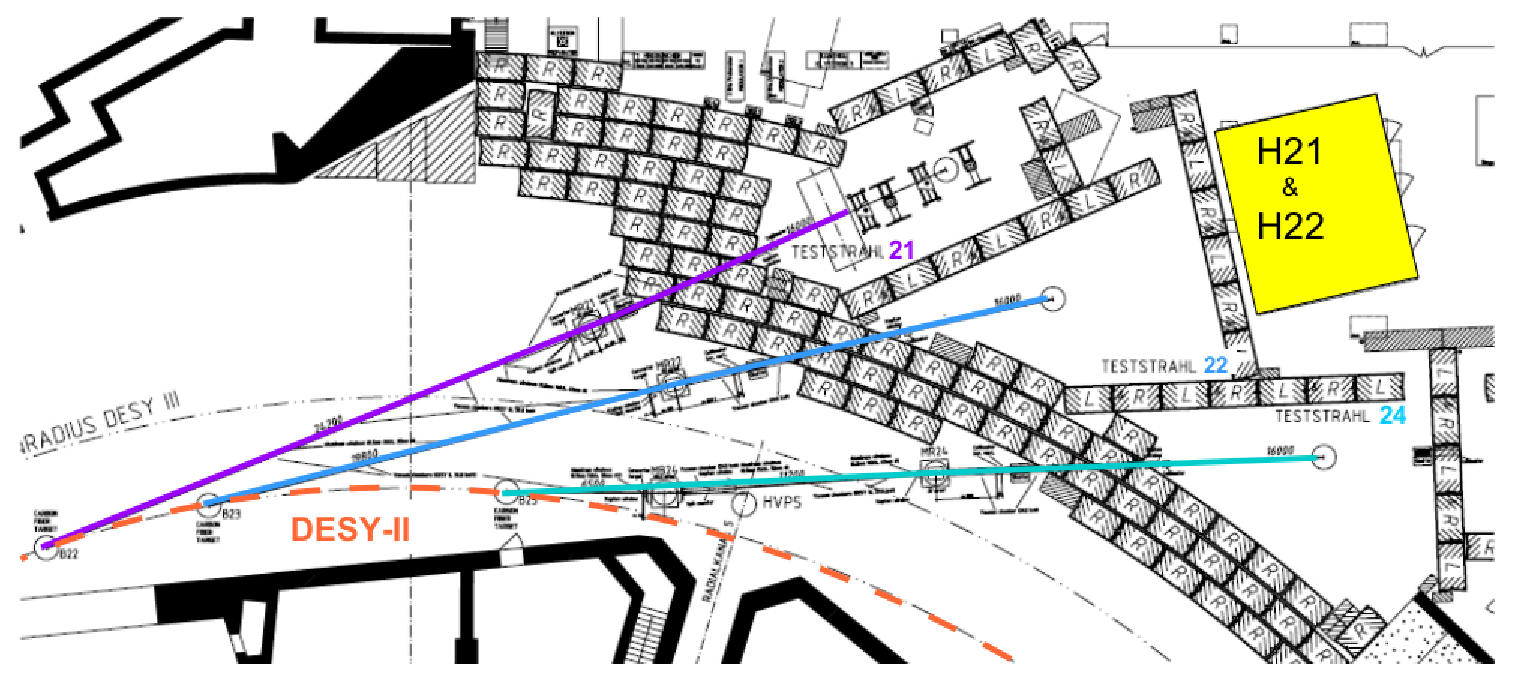
\includegraphics[width=\textwidth]{TESTBEAMS-map2.eps}
  \caption[A map of the DESY test beam lines in the DESY-II tunnel.]{A map of the DESY test beam lines in the DESY-II tunnel from 2002, which shows a state of the beam lines that deviates slightly from the current state.\cite{testbeam-web2-fig}  The evacuated beam pipes are shortened, so that currently the particles are also travelling through the air of the DESY-II tunnel.}
    \label{fig:Test Beam Lines}
\end{figure}

\subsection{The secondary target}
{\bfseries{Coordinate System ????}}
In the secondary target, the bremsstrahlung photons are converted to electron/positron pairs.  As the cross section for pair production is dependent on material and target thickness, the rate of the final test beam depends on the choice of the secondary target. The test beam users can choose from a set different converter plates cosnisting of aluminium and copper of various thicknesses.. The most commonly used converter target is the a copper target with 5\,mm thickness as it yields the highest particle rate.

Figure~\ref{fig:converter_rates} shows the comparison between the numbers of electrons and positrons simulated after the conversion of 205,500 photons in the different converters. Copper targets yield higher electron rates than the aluminium targets, and the thicker the material, the more photons are converted into electron/positron pairs. The copper wire yields the least electron/positron pairs. From the plotted numbers, the approximate conversion efficiencies were calculated and listed in Table~\ref{table:conversion_efficiency}.

\begin{figure}[htbp]
  \centering
  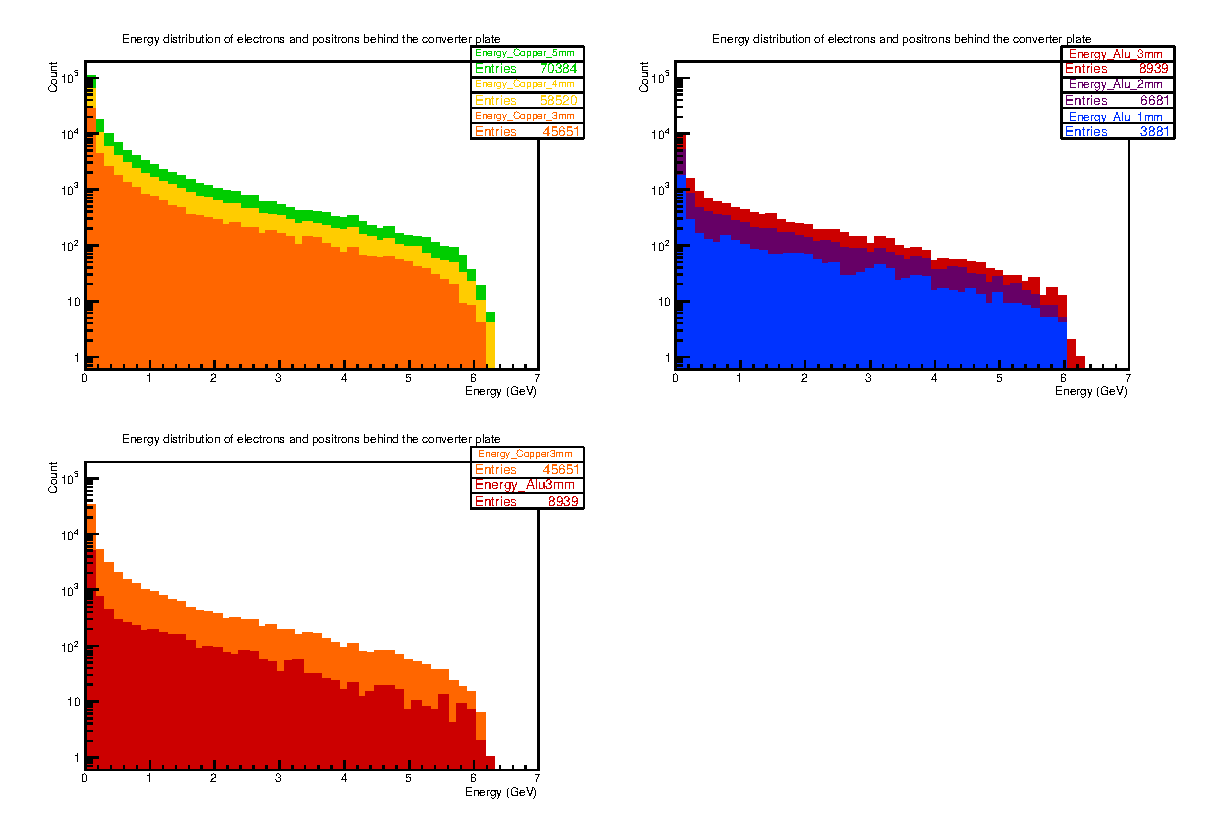
\includegraphics[width=\textwidth]{NEW_stack.eps}
  \caption[Energy distribution of electrons and positrons after photon conversion in different secondary targets of test beam line 21.]{The stacked histogram plots show the energy distribution of electrons and positrons behind the secondary target of the test beam line 21. With the comparison between the different secondary targets in respect to the material and the thickness, it is a direct comparison of their photon conversion efficiencies.}
    \label{fig:converter_rates}
\end{figure}

\begin{table}[htbp]
  \begin{center}
    \begin{tabular}{l r r@{.}l }\toprule
    \textbf{Converter} & \textbf{\#} & \multicolumn{2}{c|}{\textbf{\%}}\\ 
\midrule
    Cu 5\,mm & 70,384 & 17&13\\ 
   
    Cu 4\,mm & 58,520 & 14&24\\ 
 
    Cu 3\,mm & 45651 & 11&11\\

    Al 3\,mm & 8939 & 2&17\\

    Al 2\,mm & 6681 & 1&63\\

    Al 1\,mm & 3881 & 0&94\\
    Cu wire & 4619 & 1&12\\
    \bottomrule
    \end{tabular}
  \end{center}
  \caption[Table of simulated photon conversion efficiencies.]{Table of photon conversion efficiency to a electron/positron pair in different converter materials. To be noted is that the given efficiencies are approximated, as the mean number of 205,500 photons hitting the secondary target is taken for this calculation.}
  \label{table:conversion_efficiency}
\end{table}

\subsection{The test beam magnet}

The magnets used in the team lines are bending dipole magnets (For details 
see~\cite{DESY_TB_magnet_MR}). 
The electron/positron pairs converted from the bremsstrahlung photons in the 
secondary target enter the test beam magnet through an evacuated beam pipe, 
about 60\,cm behind the converter plate. The simulated geometry is shown in Figure~\ref{fig:3D_model_converter}.

\begin{figure}[ht]
  \centering
  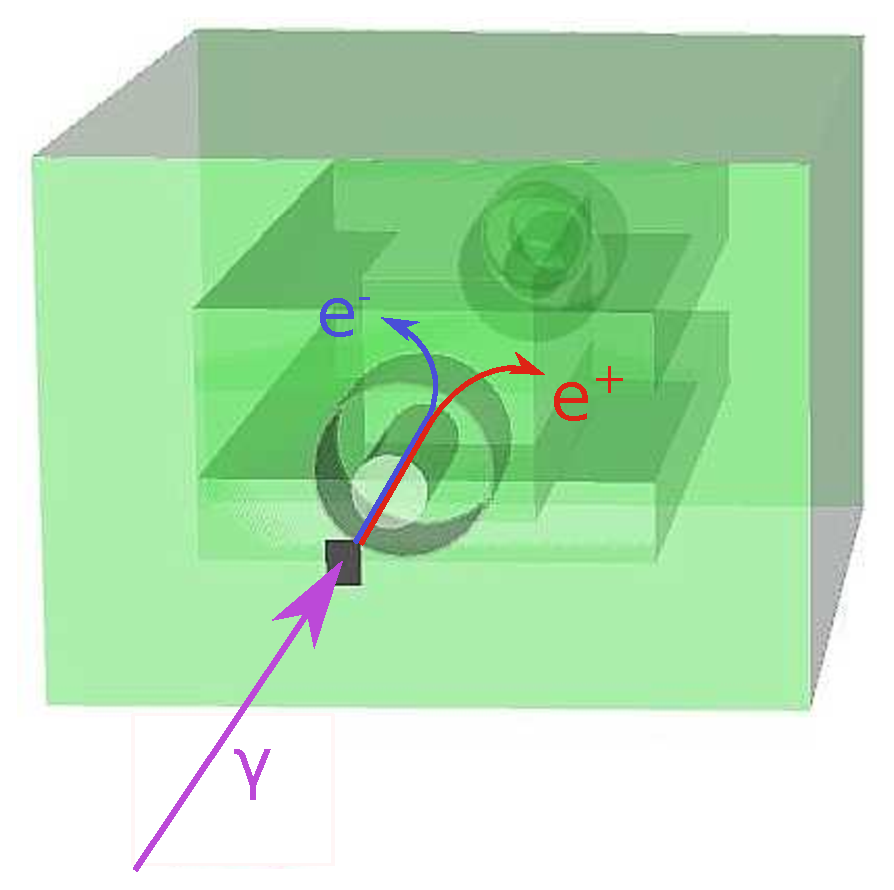
\includegraphics[width=0.45\textwidth]{3D_simulation_model_converter_particles.eps}
  \caption[3D simulation model of a converter plate in front of the dipole magnet.]{The simulated converter plate in front of the dipole magnet of the test beam line. Schematically, an electron and positron are shown  entering the dipole bending magnet and bent in opposite direction in the xz-plane.}
    \label{fig:3D_model_converter}
\end{figure}

The electron/positron beam is spread by the dipole into a particle fan in the xz-plane 
and separated by charge and energy. Neutral particles, like unconverted photons, 
 are not deflected in a magnetic field and stay on their 
initial path (in the case they are not scattered or stopped), they will leave 
the test beam magnet centrally through the exit beam pipe.\\
To separate the neutral particles from the desired electrons and positrons of 
the final test beam, the beam pipe has a small kink 15\,cm behind the test beam 
magnet. The kink angle of the pipe is 32\,mrad about the y-axis, in the positive 
x-direction. All subsequent components of the test beam line are positioned 
along this new beam path. Only charged particles with the desired momentum continue 
along the new beam path, whereas all other particles will not enter the 
subsequent beam line components. 
The particle energy can controlled by test beam user by adjusting the current of the dipole magnet.

Since the beam pipe has a radius of 5\,cm and is kinked, only the previously selected part of 
the fan enters the test beam area. The particle mometum is Gaussian distributed, where the mean 
value belongs to the particles following the ideal beam path through the centre 
of the pipe. The width of the distribution is large due to the large beam pipe aperture.
The beam size and therefore the width of the energy distribution can be reduced by two independent collimator systems, 
which can be controlled by the test beam users.
 
To illustrate the deflection of charged particles in the test beam magnet, 
Figures~\ref{fig:deflection_plot_neg/pos} show the deflection of the particles a
x-y-plane of behind the dipole magnet. The two 
separate particle fans for positively and negatively charged particles are 
clearly visible. The black circle indicate the contour of the beam pipe and only particles within
enter the beam pipe behind the magnet. The other particles will hit 
the iron surrounding of the magnet and not proceed along the beam path. Since the 
beam pipe is kinked in positive y-direction (see above), only the 
particles that are also deflected in the positive x-direction ({\bfseries x oder y} are able to 
continue on the test beam line. If the users desire positrons instead of electrons  the magnetic field 
polarity has to be reversed. 


\begin{figure}[H]
  \centering
  \begin{subfigure}[t]{0.49\textwidth}
    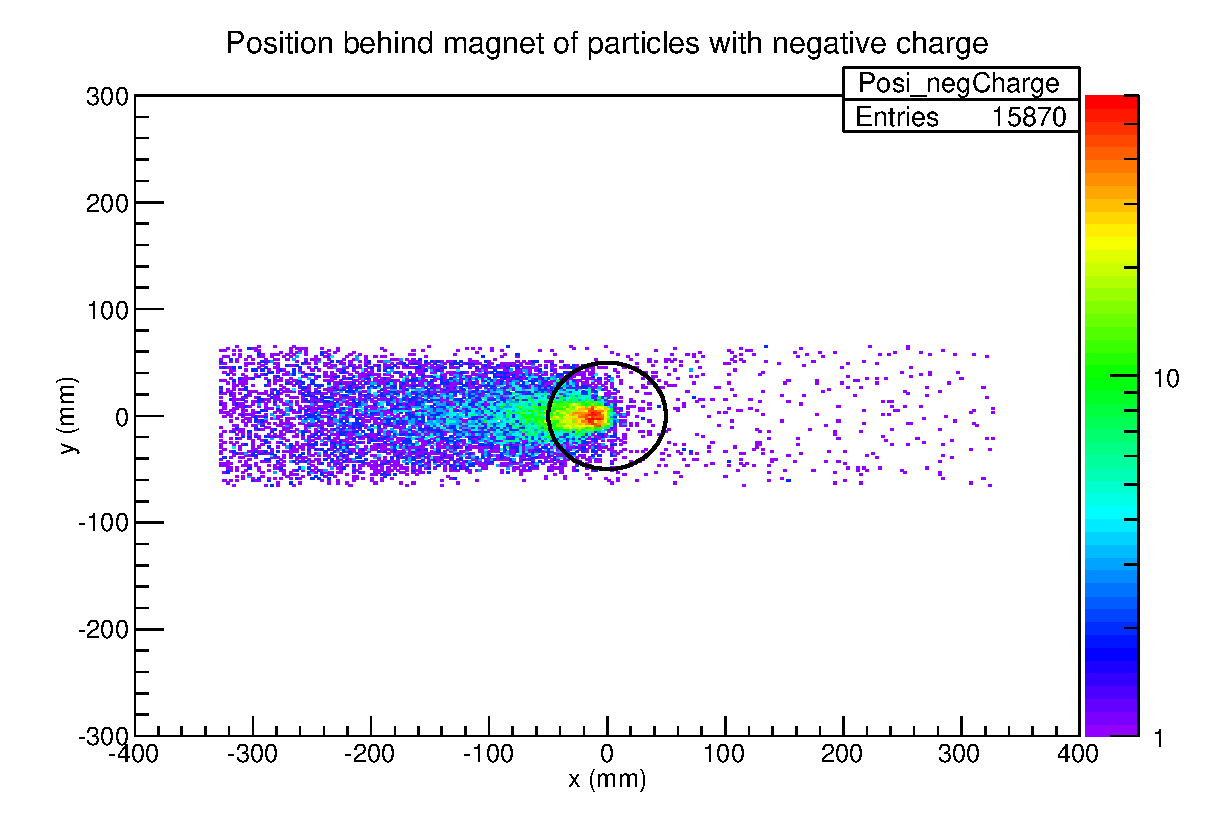
\includegraphics[width=\textwidth]{Position_negCharge_Canvas_allfiles_TBmagnet_B-0_3T.eps}
      \caption{Negatively charged particles}
  \end{subfigure}
\hfill
  \begin{subfigure}[t]{0.49\textwidth}
    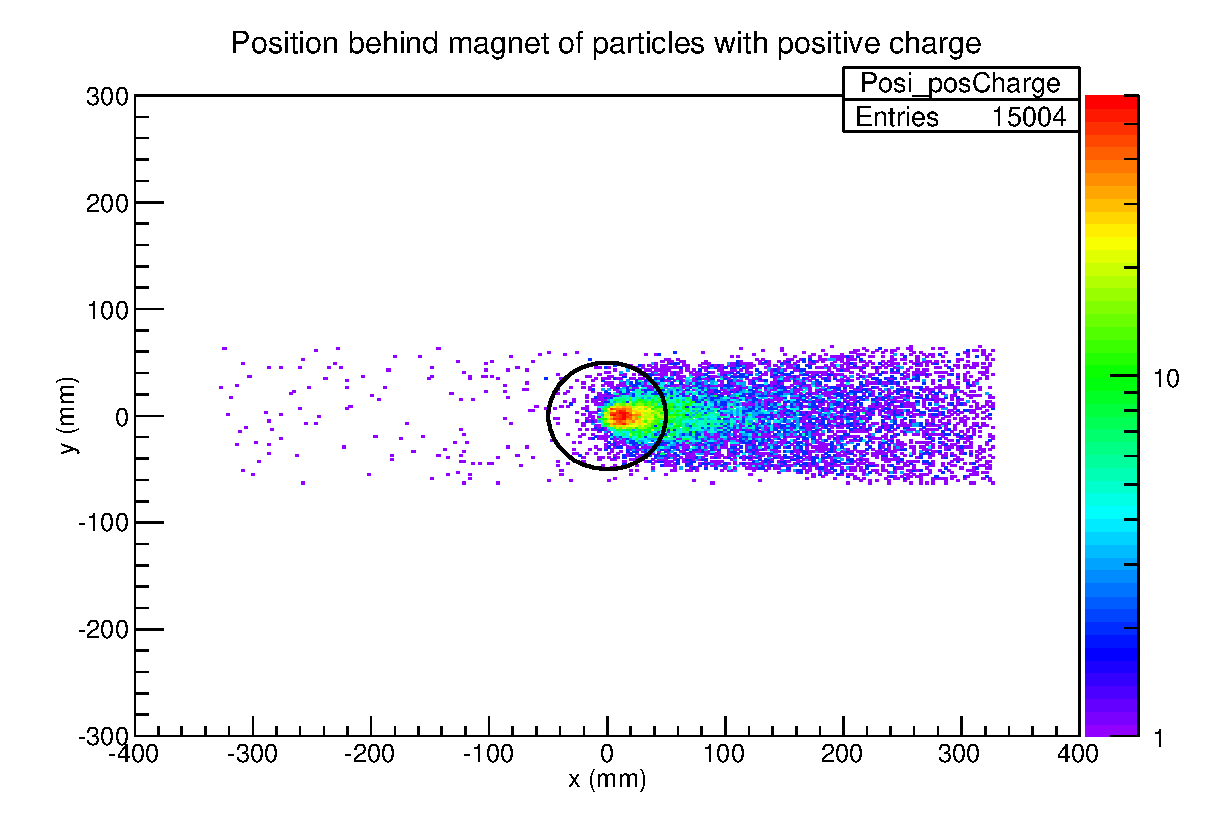
\includegraphics[width=\textwidth]{Position_posCharge_Canvas_allfiles_TBmagnet_B-0_3T.eps}
      \caption{Positively charged particles}
  \end{subfigure}
 \caption[Position plots for negatively/positively charged particles behind the test beam magnet.]{The points represent the x-/y-positions of the particles directly behind the magnet, e.g. the positions where the particles leave the magnet. The black circle illustrates the beam pipe coming out of the magnet. For the simulation, a magnetic field strength of B\,=\,-0.3\,T was chosen. The particles around the particle fan (particles with 0\,mm\,<\,x\,<\,400\,mm in Figure (a), and -400\,mm\,<\,x\,<0\,mm in Figure (b)) are scattered particles. This deviating from the particle fan is caused by particles entering the magnet with an angle to the z-axis or scattering off the material in the magnet or both.}
  \label{fig:deflection_plot_neg/pos}
\end{figure}

\subsection{The primary test beam collimator}

The test beam collimator consists of two separate collimators, a horizontal and 
vertical one. They are both built up by two tungsten blocks with variable 
distance between each other. By collimating the beam, the Gaussian energy 
distribution of the final test beam is narrowed, and the stronger the 
collimation, the smaller is the width of the distribution.\\
Figure~\ref{fig:3D_model_collimators} shows the visualised simulated model of 
the collimator with a gap size of 1\,cm, which is most commonly used.

\begin{figure}[htbp]
  \centering
  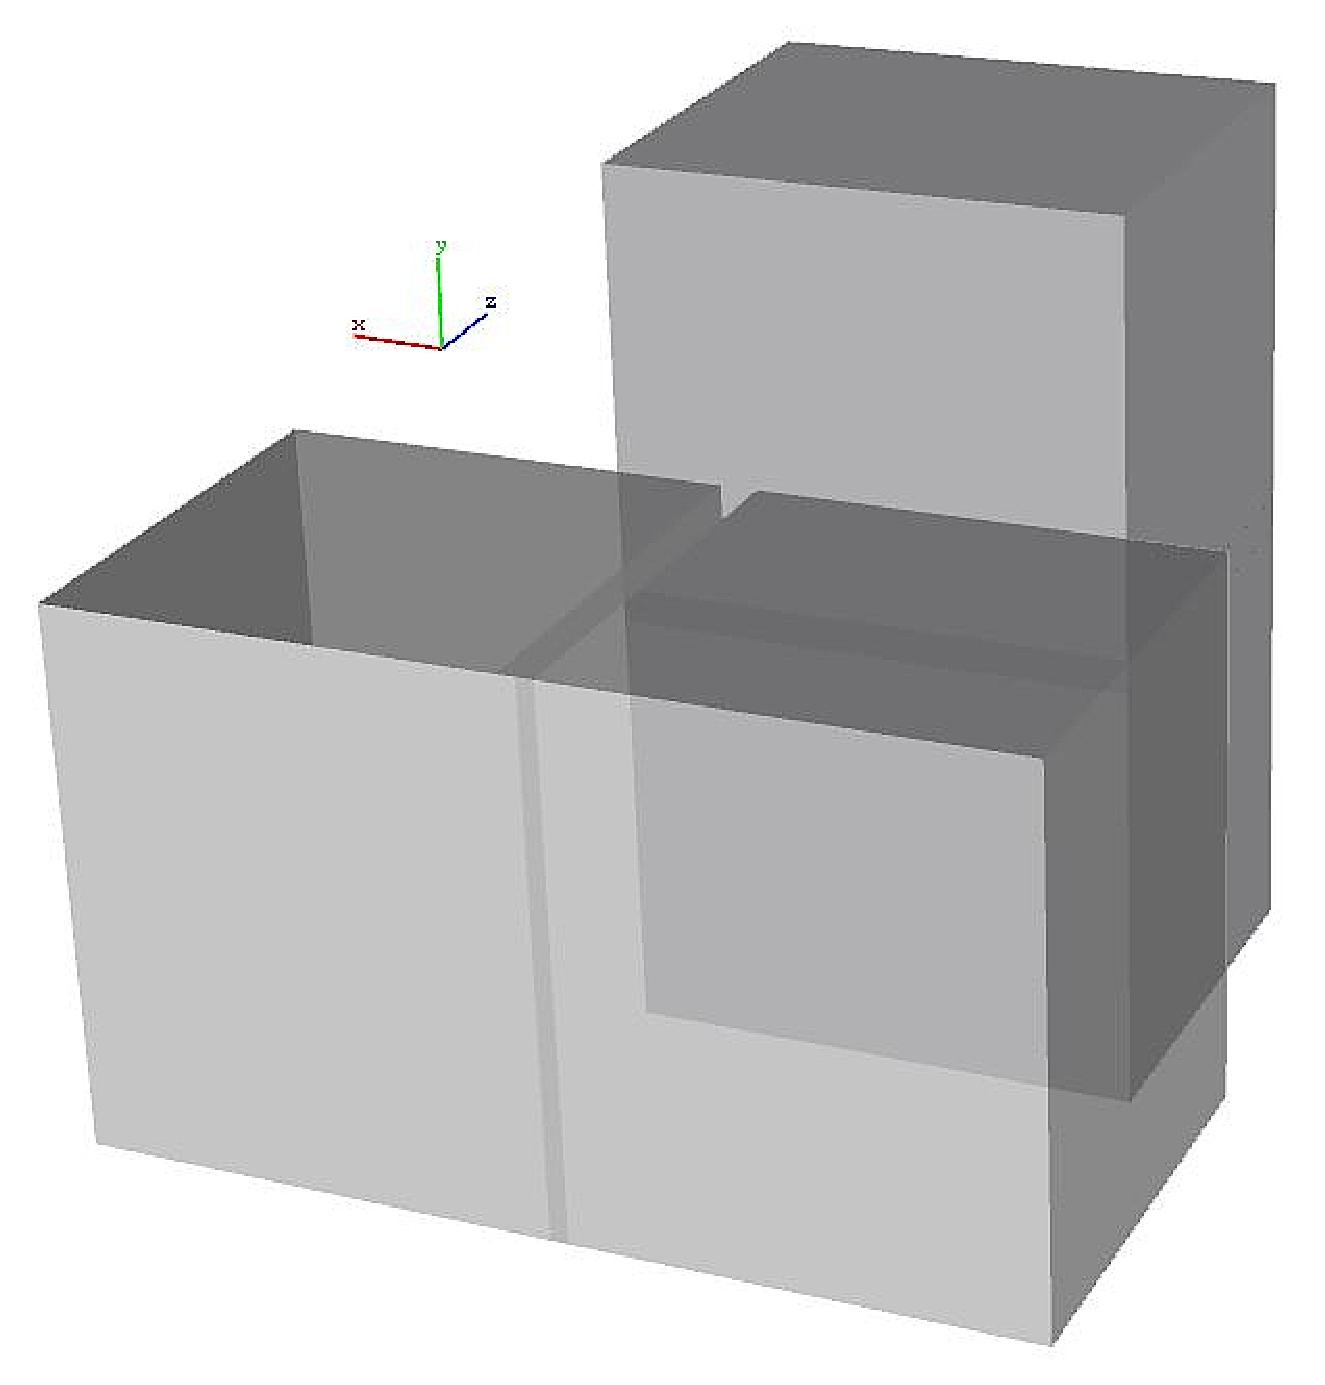
\includegraphics[width=0.35\textwidth]{3D_simulation_model_collimators.eps}
  \caption[3D simulation model of the horizontal and vertical collimators of the test beam lines.]{The simulated model of the horizontal and vertical collimators of the test beam lines are visualised with a \vrml viewer. The gap size between the tungsten blocks of both of the collimators is 1\,cm. The distance between the horizontal and the vertical collimator is about 7.9\,cm.}
    \label{fig:3D_model_collimators}
\end{figure}

\subsection{Final collimation in the test beam area}

The test beam areas are separated from the DESY-II synchrotron tunnel by a 
concrete wall, that is up to 5\,m thick. The concrete is radiation safety 
concrete with a fraction of 90\,\% iron. After the first collimation by the 
horizontal and vertical collimators, the beam continues along the evacuated beam 
pipe through the concrete wall into the test beam area. 
To illustrate the trajectory of a beam particle, the simulation of a geantino 
trajectory in the test beam line is shown in Figure~\ref{fig:TBline_trajectory}. 
A geantino is a virtual particle for transportation processes in \geant 
simulations.~\cite{Geantino}
\\In the test beam area, the test beam is again collimated by a lead collimator 
with different available hole sizes. The size of the collimator hole affects 
amongst others the number of particles and the width of the energy distribution 
of the final test beam.

\begin{figure}[htbp]
  \centering
  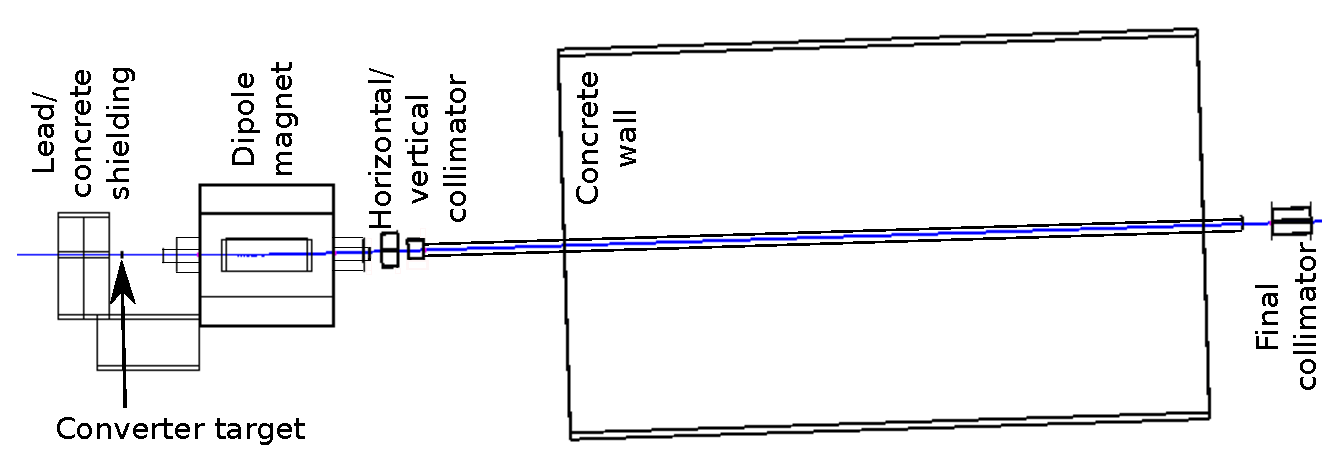
\includegraphics[width=0.9\textwidth]{TBline_with_trajectory_zoomin.eps}
  \caption[Visualisation of a geantino trajectory in the test beam line 21.]{Visualisation of the test beam line 21 with a geantino trajectory. As the xz-plane is shown with a view on top of the geometry, the geantino passes through the test beam line from the left to the right hand side.}
    \label{fig:TBline_trajectory}
\end{figure}


\chapter{Prospects, requirements and limits for the International Linear Collider}
\label{Results}
Detailed studies of different background sources for the International Linear Collider have been presented in Chapters~\ref{PairBkg},~\ref{machine_bkg}, and~\ref{BeamDumps}.
They cover the \positron\electron pair background from beam-beam interactions, the machine background from the interaction of the beam with the beam line components, and the neutron background from the ILC main beam dumps.
\\All of these background sources have been examined in extensive Monte Carlo simulation studies using various physics event generators, such as \guineapig, \mucarlo, \bdsim, and \fluka.
The impact on the \sid detector from the background particles was then simulated in the \geant based simulation tool \slic, using the \sid simulation infrastructure.
Additionally, the functionality of a vertical beam halo collimator has been tested through measurements of the machine backgrounds at the Accelerator Test Facility 2.
\\Overall, a broad range of background sources has been studied, which has brought insights of the impact of the accelerator design on the background.
The full detector simulations have then shown the effect of the background particles on the \sid detector performance.
The following sections will briefly recap and contextualize the results of the previous chapters.

\section{Keeping the detector background below the critical acceptance limit}
Achieving the ILC goal of measuring particle properties and their interactions with unprecedented precision relies on the detectors to be able to exploit their state-of-the-art technologies.
This in turn depends on clean environments for the detectors.
A balance has to be found between accelerator design and detector design optimizations, in order to minimize the detector background.
The \sid guideline for an acceptable background limit is that no more than \num{e-4} of all cells in the individual subdetectors shall be filled up with background hits above the buffer depth of the sensors.
This guideline was used throughout the chapters in order to make recommendations on acceptable background levels from the respective background sources, based on the detailed simulation studies that have been done for this thesis.

\section{Impact of the ILC running scheme on the background level}

As Chapter~\ref{PairBkg} has shown, the pair background is dependent on certain factors, such as the ILC center-of-mass energy, the number of bunches per train, and the beam parameters themselves.
These dependencies result in requirements and limits that can be formulated for the International Linear Collider.
The pair background studies done for the new proposed beam parameters for the ILC250 stage showed the effect of changes in the parameter sets on the pair background envelopes and the arising occupancy in \sid.
Three new sets ((A), (B), and (C)) had been suggested, for which the horizontal beam emittance is reduced in comparison to the original baseline parameter set.
For sets (B) and (C), the beta function values had additionally been changed.
In the \sid vertex detector, for which a minimal background level is crucial, the pair background occupancy for sets (B) and (C) exceeded the critical acceptance limit.
In set (A), the occupancy stays below the critical limit in all \sid subdetectors.
The results of this study have already been input to the ILC design decision made for the Change Request CR-0016.
Set (A) has been chosen for the new official parameter set of the ILC250 stage.

\paragraph{Possible accelerator design optimizations to constrain the background levels}

As mentioned above, design choices regarding the beam parameters effect the beam induced backgrounds.
Studying the effects on the pair background occupancies in \sid allowed to make recommendations on the design decision.
\\Also the machine background is dependent on the ILC accelerator conditions, as has been shown in Chapter~\ref{machine_bkg}.
The number of muons from the Beam Delivery System rises by a factor of three when upgrading the ILC from a center-of-mass energy of \SI{250}{\GeV} to \SI{500}{\GeV}.
Although the minimal shielding option for the muons was found to be sufficient for limiting the \sid detector occupancy, the additional shielding wall serves as a tertiary containment device, which is required due to radiation safety regulations.
\\The measurements of the machine background at the Accelerator Test Facility 2 (ATF2) have shown that the machine background is directly dependent on the beam intensity and the beam pipe vacuum pressure.
The vertical beam halo collimator, which has been tested at ATF2 regarding its functionality, has proven itself to reduce the background level at the interaction point regardless of the beam intensity or vacuum pressure conditions.
\\Chapter~\ref{BeamDumps} discussed the current ILC main beam dump designs.
Since they are based on a water vessel, the beam power can be sufficiently absorbed over a short length.
This, however, implies that the beam energy has to be dissipated effectively with the help of high-pressure water flow vortices.
Locations of high material densities lead to a high concentration of deposited energy, and to high dose rates due to the irradiation of the water and the surrounding materials. 
Even after a cooling time of one year, the dose rate in the proximity of the beam dump reaches about \SI{10}{\milli\sievert\per\second}, which tightly restricts the duration of stay for the maintenance personnel.
Additionally, the beam dumps represent another source of background for the detectors at the interaction region.
Neutrons from photonuclear interactions between the secondary particles of the developing particle showers and the water molecules can be found under every solid angle, and hence also in the backward direction towards the IP.
A simulation of the neutrons traveling back through the extraction line tunnel revealed that about \num{5.9e6} neutrons arrive at the interaction region.
A proposed solution to both of these issues is to use a gaseous beam dump instead of a water beam dump.

\section{Impact of the \sid design on the background level}

When all possible optimizations of the accelerator design have been made, the detectors have to consider the background levels in their geometric design as well as in their readout architecture.
Chapter~\ref{PairBkg} compared different \sid geometry variants with respect to their impact on the detector occupancy from the pair background.
The detectors can therefore influence the background levels themselves through various means.

\paragraph{Possible \sid design optimizations to constrain the background levels}

The detector specific anti-DiD field, for example, sweeps the pair background particles through the outgoing beam pipe, and therefore reduces the number of pairs hitting the \sid BeamCal.
This in turn also reduces the overall pair background occupancy also in the inner subdetectors.
\\In addition, the detectors have their own shielding device, Pacman, which is installed on the outside of the muon system.
The detector simulation of the beam dump neutrons arriving at the \sid detector, which has been discussed in Chapter~\ref{BeamDumps}, has proven Pacman to shield the incoming neutrons from hitting the inner subdetectors.
A proposal made in Chapter~\ref{machine_bkg} suggests to magnetize Pacman additionally in order to effectively shield also the muons coming from the Beam Delivery System.
\\All in all, the detectors have the potential to optimize their designs with respect to reducing the background levels further.
\chapter{Conclusion}
\label{Conclusion}
The International Linear Collider will be a linear \positron\electron collider at the precision frontier, and therefore complementary to the LHC.
The physics goals of the different ILC stages include measurements of the properties and the interactions of the Higgs boson and the top quark, as well as dark matter and BSM searches.
The aim for these measurements is to have unprecedented precisions.
Examples have been given in Section~\ref{ILC:physicsmotivation}, showing order of magnitude increases in precision at the ILC in comparison to the LHC.
In order to achieve such levels of precision, a balance has to be found between accelerator design and detector design optimizations with respect to minimizing the detector background.

This thesis has motivated the need for detailed background studies for the ILC.
To this end, Chapter~\ref{PairBkg} describes the beam induced \positron\electron pair background and its dependencies on ILC running schemes.
Looking at different beam parameter sets and ILC stages, the pair background was found to be a \mbox{significant} background source, which needs to be confined by both ILC and detector optimizations.
Failing to do so would mean that the pair background occupancy would negatively affect the performance of the vertex detector and the aimed-for precision measurements.

In extensive simulations, further background sources have been studied as well.
Proposed shielding options to prevent the muon machine background from the Beam Delivery System from reaching the detectors are discussed in Chapter~\ref{BDS_Muons}.
Although even the minimal shielding option shields the muons successfully from the detectors, the additional shielding wall serves as a tertiary containment device, which is required due to radiation safety regulations.

Direct measurements of machine background levels at the Accelerator Test Facility 2 have been taken for different machine conditions, in order to validate the functionality of a beam halo collimator for the ILC.
This has been done successfully, and all details on the measurements and according Monte Carlo simulation studies are presented in Chapter~\ref{machine_bkg}.

Finally, Chapter~\ref{BeamDumps} analyzes the ILC main beam dumps, which are based on water vessels.
Dumping the ILC beam causes a high radiation dose of the surroundings, restricting the duration of stay severely for the maintenance personnel.
Additionally, it creates neutrons traveling back to the interaction region, affecting the outer subdetectors of the detector experiments with respect to the detector occupancy and causing radiation damage.
As an alternative approach, gaseous beam dumps have been suggested, which show results that are orders of magnitude better.

In the process of these analyses, the impact on the \sid detector has been investigated.
By applying the \sid guideline for an acceptable background limit, the occupancies in the detector have been studied, and recommendations have been made accordingly with respect to limiting the background levels below the critical acceptance limit.
These recommendations have also been tested and have been found to be successful.
The results of the presented studies and the given recommendations are summarized in Chapter~\ref{Results}.
They are a valuable input to design decisions, and design changes based on the given recommendations to both the ILC and \sid have already been made or are currently under consideration.

Although all of the presented studies are done for the \sid detector only, the generated simulation data have been made available to the ILC community.
With a detailed understanding of the various background sources, the detector background levels can be reduced even further due to refined optimizations of the accelerator and the detectors.
This will enable the ILC and its experiments to achieve their goals of unprecedented precision measurements.

%\chapter*{Bibliography}
\addcontentsline{toc}{chapter}{Bibliography}
%\bibliography{Misc/bibliography}              %%% include the bibliography 
\printbibliography
%TODO : change the bibtex style 'misc' to 'techreport' for the SiDBkgNote as soon as it is published in a magazine  

\end{document}
